\documentclass[12pt]{article}
\usepackage[top=1in,bottom=1in,left=1in,right=1in]{geometry}
\usepackage{alltt}
\usepackage{array}	
\usepackage{graphicx}
\usepackage{tabularx}
\usepackage{verbatim}
\usepackage{setspace}
\usepackage{listings}
\usepackage{amssymb,amsmath, amsthm}
\usepackage{hyperref}
\usepackage{oz}
\usepackage[cc]{titlepic}
\usepackage{fancyvrb}
\usepackage{xcolor}
\usepackage{ulem}

\definecolor{codegreen}{rgb}{0,0.6,0}
\definecolor{codegray}{rgb}{0.5,0.5,0.5}
\definecolor{codepurple}{rgb}{0.58,0,0.82}
\definecolor{backcolour}{rgb}{0.95,0.95,0.92}

\lstdefinestyle{mystyle}{
    backgroundcolor=\color{backcolour},   
    commentstyle=\color{codegreen},
    keywordstyle=\color{magenta},
    numberstyle=\tiny\color{codegray},
    stringstyle=\color{codepurple},
    basicstyle=\ttfamily\footnotesize,
    breakatwhitespace=false,         
    breaklines=true,                 
    captionpos=b,                    
    keepspaces=true,                 
    numbers=left,                    
    numbersep=5pt,                  
    showspaces=false,                
    showstringspaces=false,
    showtabs=false,                  
    tabsize=1,
}

\lstset{style=mystyle}

\title{Concordia University\\
Department of Computer Science and Software Engineering\\
\textbf{SOEN 331:\\Formal Methods for Software Engineering}\\
\ \\
\textbf{Exercises in Z and Object-Z}}
\author{\textbf{Nathan Grenier, Nirav Patel}\\
\ \\}
\date{\today}

\begin{document}

\begin{spacing}{1.5}
	
	\maketitle
	
	\newpage
	
	\section*{PROBLEM 1 (40 pts)}
	
	Consider a system that handles railway connections as it associates (source) cities to all their corresponding destinations. The requirements of the system are as follows:
	
	\begin{enumerate}
		\item A source city may have connections to possibly multiple destination cities.
		\item Multiple source cities may share the same group of destination cities.
	\end{enumerate}
	
	We introduce the type \textit{CITY}. A possible state of the system is shown below as it is captured by variable \textit{connections}:
	
	\begin{align*}
		connections & =                                                       \\
		\{ \\
		            & Montreal \mapsto \{Ottawa, Kingston, Quebec, Halifax\}, \\
		            & Ottawa \mapsto \{Montreal, Toronto\},                   \\
		            & Toronto \mapsto \{Montreal, Ottawa\},                   \\
		            & Halifax \mapsto \{Montreal, Quebec\},                   \\
		            & Quebec \mapsto \{Montreal, Halifax\},                   \\
		            & Kingston \mapsto \{Montreal\}                           \\
		\}
	\end{align*}
	
	\begin{enumerate}
		\item (2 pts) Is \textit{connections} a binary relation? Explain why, and if so express this formally.
        \newline
        
        \noindent \underline{Solution}:

		      Yes, the variable $connections$ represents a binary relation. A binary relation is a set of ordered pairs where each pair consists of two elements. In this case, the pairs in $connections$ are formed by associating a source city with its corresponding set of destination citites.
		      
		      Formally, a binary relation $R$ from set $A$ to set $B$ is defined as a subset of the cartesian product $A\times B$. In this context, the set of connections can be expressed formally as:
		      
		      $$connections \subseteq \{(source, destination) | source \in CITY, destination \in CITY\}$$
		      
		      Therefore, the variable $connections$ conforms to the definition of a binary relation as it relates source cities to their respective destination cities in pairs.
		          
		\item (2 pts) In the expression $connections \in (...)$, what would RHS be?
		      
		      The right-hand side would be the set of all possible binary relations on the set of cities, denoted as '\texttt{CITY}'.
		      
		      Formally, the right-hand side can be represented as:
		      
		      $$(CITY \times \mathcal{P}(CITY))$$
		      
		      Where:
		      \begin{itemize}
		      	\item '\texttt{CITY}' is the set of all cities
		      	\item '$\mathcal{P}(CITY)$' is the power set of '\texttt{CITY}', which represents the set of all possible subsets of '\texttt{CITY}'.
		      	\item '\texttt{CITY}$\times \mathcal{P}$(\texttt{CITY})' is the Cartesian product of '\texttt{CITY}' and '$\mathcal{P}$(\texttt{CITY})', which represents the set of all ordered pairs '$(source, destinations)$' where '$source$' is a city and '$destinations$' is a set of cities.
		      \end{itemize}
		      
		      Therefore, the expression '$connections \in (CITY, \mathcal{P}(CITY))$' means that the $connections$ variable is an element of the set of all binary relations on the set of cities.
		      
		\item (2 pts) Is \textit{connections} a function? If so, define the function formally, and reason about the properties of injectivity, surjectivity, and bijectivity.
		      
		      To determine if \textit{connections} is a function, we need to ensure that each source city maps to exactly one set of destination cities.
		      
		      We see that each source city (e.g., Montreal, Ottawa, Toronto, Halifax, Quebec, Kingston) maps to exactly one set of destination cities, satisfying the definition of a function.
		      
		      Now, let's define the function formally:
		      
		      Let $f$ be the function representing the railway connections, where:
		      
		      \begin{itemize}
		      	\item Domain (\texttt{Dom}($f$)): Set of source cities.
		      	\item Codomain (\texttt{Cod}($f$)): Set of sets of destinations cities.
		      	\item $f(x)$: Set of destination cities connected to the source city $x$.
		      \end{itemize}
		      
		      Formally:
		      $$f(x)=\text{Set of destination cities connected to source city }x$$
		      
		      We then analyze whether the function is injective, surjective, and bijective:
		      
		      \begin{enumerate}
		      	\item Injectivity: The function is injective if each source city maps to a unique set of destination cities. In this case, it's not injective because multiple source cities may share the same group of destination cities.
		      	\item Surjectivity: The function is surjective if every set of destination cities is mapped to by some source city. Since there can be multiple source cities mapping to the same group of destination cities, it is surjective.
		      	\item Bijectivity: The function is bijective if it is both injective and surjective. Since it's not injective but surjective, it's not bijective.
		      \end{enumerate}
		      
		      In conclusion, the \textit{connections} variable represents a function, but it is not injective or bijective, only surjective.
		      
		\item (2 pts) Describe the meaning and evaluate the following expression:
		      
		      \indent $\{Montreal, Halifax\} \: \triangleleft \: connections$
		      
		      The symbol $\triangleleft$ denotes the domain restriction operator. When applied to a function or a relation, it restricts the domain of a function to a specified subset.
		      
		      In the expression $\{Montreal, Halifax\} \: \triangleleft \: connections$, we are restricting the domain of the function represented by $connections$ to the set $\{Montreal, Halifax\}$.
		      
		      We are essentially interested in the subset of the connections that involve either Montreal or Halifax as the source city.
		      
		      We evaluate the expression:
		          
		      \begin{align*}
		      	Montreal & \mapsto \{Ottawa, Kingston, Quebec, Halifax\}, \\
		      	Halifax  & \mapsto \{Montreal, Quebec\}                   
		      \end{align*}
		      
		      So, after the domain restriction, we only have connections involving Montreal and Halifax as source cities.
		      
		      In conclusion, the expression $\{Montreal, Halifax\} \triangleleft connections$ yields the connections from Montreal and Halifax to their respective destination cities.
		      
		\item (2 pts) Describe the meaning and evaluate the following expression:
		      
		      \indent $connections \: \triangleright \: \{\{Montreal, Halifax\}\}$
		      
		      The symbol $\triangleright$ represents the range restriction operator. When applied to a function, it restricts the range of the function to a specified subset.
		      
		      In the expression $connections \: \triangleright \: \{\{Montreal, Halifax\}\}$, we are restricting the range of the function represented by $connections$ to the set containing the destinations Montreal and Halifax.
		      
		      We evaluate the expression:
		      
		      $$Quebec \mapsto \{Montreal, Halifax\}$$
		      
		      So, after the range restriction, we only have connections where the destination is either Montreal or Halifax.
		      
		      In conclusion, the expression $connections \: \triangleright \: \{\{Montreal, Halifax\}\}$ yields the connections from source cities that map to the destinations Montreal and Halifax.
		          
		\item (2 pts) Describe the meaning and evaluate the following expression:
		      
		      $\{Montreal, Quebec, Halifax\} \: \ndres \: connections$
		      
		      The symbol $\ndres$ represents the domain subtraction or domain anti-restriction operator. When applied to a function or a relation, it removes a specified subset from the domain of the function/relation.
		      
		      In the expression $\{Montreal, Quebec, Halifax\} \: \ndres \: connections$, we are subtracting the set  $\{Montreal, Quebec, Halifax\}$ from the domain of the function $connections$.
		      
		      We evaluate the expression:
		      
		      \begin{align*}
		      	Ottawa \mapsto \{Montreal, Toronto\}, \\
		      	Toronto \mapsto \{Montreal, Ottawa\}, \\
		      	Kingston \mapsto \{Montreal\}         
		      \end{align*}
		      
		      So, after the domain subtraction, we only have connections originating from Ottawa, Toronto, and Kingston.
		      
		      In conclusion, the expression $\{Montreal, Quebec, Halifax\} \: \ndres \: connections$ yields the connections excluding those originating from Montreal, Quebec, and Halifax.
		      
		\item (2 pts) Describe the meaning and evaluate the following expression:
		      
		      $connections \: \rsub \: \{\{Ottawa, Kingston, Quebec, Halifax\},\{Montreal, Ottawa\},\{Montreal\}\}$
		      \newline
		      The symbol $\rsub$ represents the range subtraction operator. When applied to a function, it removes a specified subset from the range of the function.
		      
		      In the expression $connections \: \rsub \: \{\{Ottawa, Kingston, Quebec, Halifax\},\{Montreal, Ottawa\},\{Montreal\}\}$, we are subtracting the set containing various sets of destinations from the range of the function represented by $connections$.
		      
		      We evaluate the expression:
		      
		      \begin{align*}
		      	Ottawa \mapsto \{Montreal, Toronto\}, \\
		      	Halifax \mapsto \{Montreal, Quebec\}, \\
		      	Quebec \mapsto \{Montreal, Halifax\}  
		      \end{align*}
		      
		      So, after the range subtraction, we only have connections starting from Ottawa, Halifax and Quebec.
		      
		      In conclusion, the expression $connections \: \rsub \: \{\{Ottawa, Kingston, Quebec, Halifax\},\{Montreal, Ottawa\},\{Montreal\}\}$ yields the connections excluding those leading to the sets defined in the expression.
		      
		\item (2 pts) Describe the meaning and evaluate the following expression that forms a post-condition to some operation:
		      
		      \begin{align*}connections'=connections \: \oplus \: & \{  \\
		      	            & Halifax \mapsto \{Montreal, Charlottetown, Quebec\},    \\
		      	            & Charlottetown \mapsto \{Halifax\}                       \\
		      	\}          & \end{align*}                                            \newline
		      	
		      	The expression given represents a post-condition for an operation involving the variable $connections$. The operator being used here is the relational overriding operated denoted by $\oplus$. This operator combines two relations, where the right-hand side relation takes precedence over the left-hand side in case of conflicting keys.
		      	
		      	After evaluating this expression with the overriding operator:
		      	
		      	\begin{enumerate}
		      	\item The existing entry for Halifax in $connections$ will be replaced with the new set of destinations: $\{Montreal, Charlottetown, Quebec\}$.
		      	\item A new entry for Charlottetown with destinations $\{Halifax\}$ will be added to $connections$.
		      	\end{enumerate}
		      	
		      	The resulting updated $connections$ will be:
		      	    
		      	\begin{align*}
		      	connections & =                                                       \\
		      	\{ \\
		      	            & Montreal \mapsto \{Ottawa, Kingston, Quebec, Halifax\}, \\
		      	            & Ottawa \mapsto \{Montreal, Toronto\},                   \\
		      	            & Toronto \mapsto \{Montreal, Ottawa\},                   \\
		      	            & Halifax \mapsto \{Montreal, Charlottetown, Quebec\},                                 \\
		      	            & Quebec \mapsto \{Montreal, Halifax\},                   \\
		      	            & Kingston \mapsto \{Montreal\}                           \\
                            & Charlottetown \mapsto \{Halifax\}
                                              \\
		      	\}
		      \end{align*}
		      
		\item (6 pts) Assume that we need to add a new entry into the database table represented by \textit{connections}. We have decided \underline{not} to deploy a precondition. What could be the consequences to the system if we deployed a) \textbf{set union} and b) \textbf{relational overriding}?\newline

        \begin{enumerate}
            \item Set Union:
            If set union is deployed without a pre-condition when adding a new entry to the $connections$ database table, the consequences could include:

            \begin{itemize}
                \item \textbf{Duplication of Data}: Without a precondition, set union may lead to duplicate entries being added to the database. This can result in inefficiencies and potential data inconsistencies.
                \item \textbf{Increased Complexity}: The set union operation may add unnecessary complexity to the system, especially if it allows for redundant or conflicting data entries.
                \item \textbf{Potential Data Integrity Issues}: Inconsistent data entries may arise if set union is used without proper checks, leading to data integrity issues within the system.  
            \end{itemize}

            \item Relational Overriding:
            \begin{itemize}
                \item \textbf{Loss of Existing Data}: Relational overriding will replace existing data without considering any conditions. This can lead to the loss of valuable information if not handled carefullly.

                \item \textbf{Potential Data Loss}: If relational overriding is applied without caution, it can overwrite critical information unintentionally, resulting in data loss and inconsistencies.

                \item \textbf{Inconsistencies in Data}: Without a precondition, relational overriding may introduce inconsistencies in the database by replacing existing connections with new ones without proper validation.
            \end{itemize}
        \end{enumerate}

         In both cases, deploying these operations without preconditions can introduce risks to the system's data integrity, consistency, and overall functionality.
         
		\item (2 pts) Consider operation \textit{AddOperation} to \textbf{add a new entry} to the table, defined by the following pair of assertions.
		      
		      \begin{align*}
		      	  & city? \: \notin \: \texttt{dom } connections                           \\
		      	  & connections' = connections \: \cup \: \{city? \mapsto destinations?\} 
		      \end{align*}
		      
		      What would be the result of the call \texttt{AddConnection(Montreal, (Boston, NYC))}, and in the case of failure, whom should we blame and why?\newline

            Given the call \texttt{AddConnection(Montreal, (Boston, NYC))}, let's evaluate it step by step:


            \begin{enumerate}
                \item Check if Montreal is not already in the domain of connections. Since Montreal is present in the domain, the first assertion fails.

                \item Since the first assertion fails, the operation cannot proceed to update the connections. Therefore, the call to \texttt{AddConnection(Montreal, (Boston, NYC))} fails.
            \end{enumerate}

            If this operation fails, the blame would typically fall on the caller of the function, who invoked the \texttt{AddConnection} function with a city that already exists in the domain of connections. It suggests that the caller did not properly check whether the city being added already exists in the system, leading to a violation of the precondition specified by the first assertion. Therefore, the caller should be responsible for handling such cases or ensuring that only valid data is passed to the \texttt{AddConnection} function.
            
		\item (2 pts) Consider the following modification to the postcondition of \textit{AddOperation}:
		      
		      $$connections'=connections \: \oplus \: \{city? \mapsto destinations?\}$$
		      
		      What would be the result of the call \texttt{AddConnection(Kingston, (Boston,NYC)}? In the absence of a precondition, can relational overriding unintentionally capture the intent of the operation? \newline
        
        The modified postcondition for the \textit{AddOperation} utilizes relational overriding ($\oplus$) to update the connections. It specifies that the new entry $city? \: \mapsto \: destinations?)$ should be added to the existing connections, overriding any existing mapping for the same city if it exists.

        Now, let's consider the call \texttt{AddConnection(Kingston, (Boston, NYC))}:

        \begin{enumerate}
            \item Since Kingston is not in the domain of connections, the operation can proceed without any conflict.

            \item The postcondition specifies that the connections should be updated using relational overriding, meaning that if Kingston already exists in the connections, its destinations will be replaced with the new destinations (Boston, NYC). If Kingston does not exist in the connections, a new entry will be added for it.
        \end{enumerate}

        In this case, since Kingston is not already in the connections, the postcondition simply adds a new entry for Kingston mapped to the destinations (Boston, NYC).

        In the absence of a precondition, relational overriding can unintentionally capture the intent of the operation if there are conflicting entries. For example, if Kingston already existed in the connections with different destinations, the use of relational overriding would replace those destinations with the new ones (Boston, NYC), potentially overriding the existing connections unintentionally.
        
        Therefore, careful consideration should be given to the potential consequences of using relational overriding without a precondition to ensure that it aligns with the intended behavior of the operation.
  
        \item (3 pts) Consider the following state schema in the Z Specification Language:

        \begin{schema}{RailwayManagement}
        cities~:~\mathcal{P}CITY\\
        connections~:~CITY\nrightarrow\mathcal{P}CITY\\
        \where
        cities=\texttt{dom }connections
        \end{schema}
		      
        Define the schema for operation $GetDestinations$ which returns all destinations for one given city.

        To define the schema for the operation $GetDestinationsGetDestinations$, which returns all destinations for one given city, we can use the Z notation. The schema will take a city as input and return its corresponding set of destinations. Here's how we can define it:

        \begin{schema}{GetDestinations}
        \Delta RailwayManagement \\
        city? : CITY \\
        destinations! : \mathcal{P}CITY \\
        \where
        city? \in cities \\
        destinations! = connections(city?) \\
        \end{schema}

        In this schema:
        \begin{itemize}
            \item $GetDestinationsGetDestinations$ represents the operation schema.
            \item $\triangle$ RailwayManagement denotes that this operation may update the state of the system represented RailwayManagement.
            \item $city?$ is an input variable representing the city for which destinations are requested
            \item $destinations!$ is an output variable representing the set of destinations corresponding to the input city.
            \item The where clause ensures that the input city ($city?$) is a valid city in the system (i.e., it exists in the set cities).
            \item The assignment $destinations!=connections(city?)$ retrieves the set of destinations for the given city from the connections mapping.
        \end{itemize}

        This schema ensures that the operation $GetDestinations$ operates correctly within the context of the $RailwayManagement$ state schema, returning the set of destinations for a given city.
		      
		\item (1 pt) (\textbf{PROGRAMMING}) Define global variables $connections$ in Common LISP and populate it with some sample data. Demonstrate that the variable indeed contains the ordered pairs as shown above.

        \lstinputlisting[language=Lisp]{code/connections-1-13.lisp}

        We explain a basic rundown of the code:

        \begin{enumerate}
            \item The code begins by initializing the global variable *connections* to an empty list using defvar. This variable will store the railway connections data.
            \item The add-connection function is defined to add a new connection to the *connections* variable. It takes two arguments: source, representing the source city, and destinations, representing a list of destination cities. It uses push to add a new cons cell representing the connection to the *connections* list.
            \item  The initialize-connections function is defined to populate the *connections* variable with sample data. It sets *connections* to a list of cons cells, each representing a connection from a source city to its corresponding destinations.
            \item The display-connections-with-arrows function is defined to visually display the connections stored in the *connections* variable. It iterates over each connection in *connections*, extracting the source city and its destinations, and prints them with arrows separating the source city from its destinations.
            \item Finally, the code calls the initialize-connections function to populate the *connections* variable with sample data and then calls the display-connections-with-arrows function to display the contents of *connections* in a visually formatted way with arrows.
        \end{enumerate}

        \begin{figure}[htp]
            \centering
            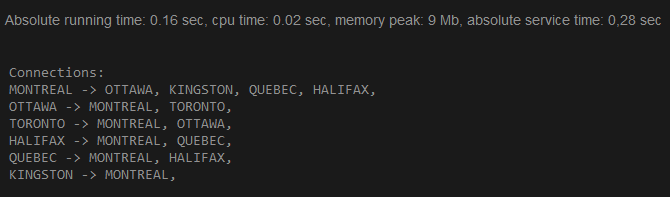
\includegraphics{static/connections-1-13.PNG}
            \caption{Environment Interaction for Question 1 - Part 13}
            \label{fig:figure}
        \end{figure}
		      
		\item (3 pts) Describe how you would validate variable $connections$ , i.e. how to show that it holds a function.

        To validate that the variable $connections$ holds a function, we need to verify that it satisfies the properties of a mathematical function. In mathematical terms, a function is a relation between a set of inputs (the domain) and a set of possible outputs (the codomain), such that each input is related to exactly one output.

        Here's how we can validate variable $connections$ to ensure it holds a function:

        \begin{enumerate}
            \item \textbf{Domain Check}: Ensure that each source city in the domain of connections is associated with at least one destination city. This ensures that every input (source city) has a corresponding output (destination city).
            \item \textbf{Unique Outputs}: Ensure that each source city is associated with a unique set of destination cities. In other words, there are no duplicate entries for the same source city. This ensures that each input is related to exactly one output.
            \item \textbf{Consistency}: Ensure that the relation is consistent, meaning that if a source city $s$ is associated with a destination city dd, then dd must be present in the domain of $connections$ with $s$ as one of its destinations. This ensures that the relation does not contain contradictory information.
            \item \textbf{No Extra Entries}: Ensure that there are no extra entries in $connections$ that do not conform to the function's definition. This means ensuring that every key-value pair in $connections$ adheres to the function's mapping rules.
        \end{enumerate}
        
		\item (3 pts) (\textbf{PROGRAMMING}) Define a predicate function, \texttt{isfunctionp}, in Common Lisp that reads a variable like $connections$ and indicates if the variable corresponds to a function or not.

        \lstinputlisting[language=Lisp]{code/isFunctionp-1-15.lisp}

        We describe a basic run-down of the code:
        \begin{enumerate}
            \item The \texttt{isFunction} function checks whether a given variable corresponds to a function.
            \item It checks if the variable is a list (\texttt{listp}), ensuring it has the structure of a function.
            \item It verifies if every element of the list is a cons cell (\texttt{consp}), ensuring each element is a key-value pair.
            \item It checks if each cons cell consists of a symbol as the key and a list as the value, as expected for a function.
            \item Example 1 demonstrates a variable ($*connections-function*$) that corresponds to a function, with a list of key-value pairs.
            \item Example 2 demonstrates a variable ($*connections-nonfunction*$) that does not correspond to a function, being just a list of symbols without the key-value pair structure.
        \end{enumerate}

        \begin{figure}[htp]
            \centering
            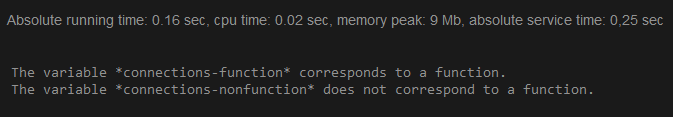
\includegraphics{static/isFunctionp-1-15.PNG}
            \caption{Environment Interaction for Question 1 - Part 15}
            \label{fig:figure}
        \end{figure}
        
		\item (2 pts) (\textbf{PROGRAMMING}) Define function $getDestinations$ in Common LISP.

        \lstinputlisting[language=Lisp]{code/getDestinations-1-16.lisp}

        We explain a basic rundown of the code:
        \begin{enumerate}
            \item The $getDestinations$ function takes two arguments: $city$, the city for which destinations are to be retrieved, and $connections$, the list of connections.
            \item Inside the function, it uses the $assoc$ function to search for the $city$ in the $connections$ list and retrieve the corresponding cons cell.
            \item Then, it uses $cdr$ to extract the destinations from the cons cell.
            \item Finally, it returns the list of destinations for the given city.
            \item Example usage demonstrates how to use the $getDestinations$ function with the $*connections*$ variable to retrieve destinations for Montreal and Ottawa.
        \end{enumerate}

        \begin{figure}[htp]
            \centering
            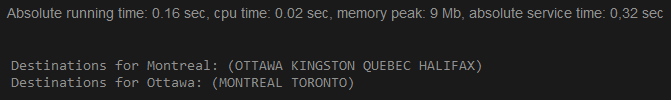
\includegraphics{static/getDestinations-1-16.PNG}
            \caption{Environment Interaction for Question 1 - Part 16}
            \label{fig:figure}
        \end{figure}
		           
	\end{enumerate}

    \section*{PROBLEM 2 (50 pts)}

    Consider an airport management system. Each airport has a unique id (e.g. Montreal:YUL).
    Let us introduce the types AIRPORT and CITY . We also introduce variable airports that
    contains associations between airport id's and their corresponding host cities. A possible
    state of the system is shown below:
    \begin{align*}
        \text{airports} = \{
        & \text{YUL} \mapsto \text{Montreal}, \\
        & \text{LCY} \mapsto \text{London UK}, \\
        & \text{LHR} \mapsto \text{London UK}, \\
        & \text{MIL} \mapsto \text{Milan}, \\
        & \text{SFO} \mapsto \text{San Francisco}, \\
        & \text{SDQ} \mapsto \text{Santo Domingo} \\
        \}
    \end{align*}

    \begin{enumerate}
        \item (1 pt) (PROGRAMMING) Define global variable airports in Common LISP and
        populate it with the above data. Demonstrate that the variable indeed contains the
        ordered pairs as shown above.

        \underline{Solution}:
        \lstinputlisting[language=Lisp]{code/airports-2-1.lisp}

        \begin{figure}[htp]
            \centering
            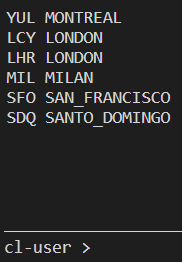
\includegraphics{static/airports-2-1.PNG}
            \caption{Output of Question 2 - Part 1}
        \end{figure}

        \item (2 pts) Provide a declaration of variable $monitored$ that holds all airport id's.
        
        \underline{Solution}:
        $$monitored : \mathcal{P}(AIRPORT)$$ 
        \begin{verbatim}
            monitored = {YUL, LCY, LHR, MIL, SFO, SDQ}
        \end{verbatim}

        \item (3 pts) What kind of variable is airports? Provide a formal definition together with
        any and all applicable properties.

        \underline{Solution}:
        
        $airports$ is a partial injective function from the set of airport ids to the set of cities. It is defined as follows:
        $$airports : AIRPORT \pinj CITY$$
        \begin{schema}{Airports}
            city : \mathcal{P}(CITY) \\
            airportId : \mathcal{P}(AIRPORT) \\
            airports : airportId \pinj city \\
            \where
            \forall a_i, a_j : airports \bullet a_i.airportId \neq a_j.airportId \\
            \forall a_i, a_j : AIRPORT \bullet a_i \neq a_j \implies a_i.airportId \neq a_j.airportId
        \end{schema}

        \item (3 pts) Describe what data structure you would deploy to model variable airports.
        Note that you may not use a Dictionary. Should this be an ordered or an unordered
        structure? Discuss

        \underline{Solution:}
        A pair of sets, one containing the airports and another the cities.
        It should be unordered because each airport must have a unique id, and the order of insertion doesn't matter.

        \item (4 pts) Provide a formal specification of the state of the system in terms of a Z specification schema
        
        \underline{Solution:}
        \begin{schema}{AirportManagement}
            airports : AIRPORT \pinj CITY \\
            monitored : \mathcal{P}(AIRPORT) \\
            \where
            \text{dom}(airports) = monitored
        \end{schema}

        \item (6 pts) Provide a schema for operation AddAirportOK that adds a new airport to the
        system. With the aid of success and error schema(s), provide a definition for operation
        AddAirport that the system will place in its exposed interface.
        
        \underline{Solution:}
        \begin{schema}{AddAirportOK}
            \Delta AirportManagement \\
            airport? : AIRPORT \\
            city? : CITY \\
            \where
            airport? \notin \text{dom}(airports) \\
            airports' = airports \cup \{airport? \mapsto city?\} \\
        \end{schema}
        $$MESSAGE ::= ok | error.$$

        \begin{schema}{Success}
            \Xi AirportManagement \\
            response! : MESSAGE \\
            \where
            airport! = \, 'ok' \\
        \end{schema}

        \begin{schema}{AirportAlreadyExists}
            \Xi AirportManagement \\
            airport? : AIRPORT \\
            response! : MESSAGE \\
            \where
            airport? \in \text{dom}(airports) \\
            response! = \, 'error' \\
        \end{schema}
        $$AppAirpot \, \hat{=} \, (AddAirportOk \land Success) \oplus AirportAlreadyExists$$
    \end{enumerate}
\end{spacing}

\end{document}